\begin{figure}[h!p]
  \begin{center}
    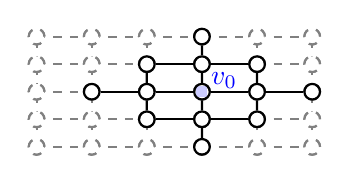
\begin{tikzpicture}[thick, scale = 0.7]
      \tikzstyle{every node} = [inner sep = 2pt];
      \foreach \x in {0,...,5}{
        \foreach \y in {0,...,4}{
          \node [draw, circle, dashed, black!50] at (\x, \y/2) {};
        }
      }
      \foreach \x in {0,...,4}{
        \foreach \y in {0,...,4}{
          \path[-]
          (\x,\y/2) edge[dashed, black!50] (\x+1,\y/2);
        }
      }
      \foreach \x in {0,...,5}{
        \foreach \y in {0,...,3}{
          \path[-]
          (\x,\y/2) edge[dashed, black!50] (\x,\y/2 + 1/2);
        }
      }
      \foreach \x in {0,...,5}{
        \foreach \y in {0,...,4}{
          \node [draw = black!50, dashed, circle,fill=white] at (\x, \y/2) {};
        }
      }
      \node[fill=blue!20!white] at (3,1){};
      \node at (3.4,1.2){\textcolor{blue}{$v_0$}};
      \node(bb) [draw, circle] at (3, 0) {};
      \node(s) [draw, circle] at (3, 1) {};
      \node(b) [draw, circle] at (3, 0.5) {};
      \node(u) [draw, circle] at (3, 1.5) {};
      \node(uu) [draw, circle] at (3, 2) {};
      \node(l) [draw, circle] at (2, 1) {};
      \node(lb) [draw, circle] at (2, 0.5) {};
      \node(lu) [draw, circle] at (2, 1.5) {};
      \node(r) [draw, circle] at (4, 1) {};
      \node(rb) [draw, circle] at (4, 0.5) {};
      \node(ru) [draw, circle] at (4, 1.5) {};
      \node(ll) [draw, circle] at (1, 1) {};
      \node(rr) [draw, circle] at (5, 1) {};
      \path[]
      (s) edge (u)
      edge (l)
      edge (b)
      edge (r)
      (l) edge (ll)
      edge (lu)
      edge (lb)
      (r) edge (rr)
      edge (ru)
      edge (rb)
      (u) edge (uu)
      edge (lu)
      edge (ru)
      (b) edge (bb)
      edge (lb)
      edge (rb);
    \end{tikzpicture}
  \end{center}
  \caption{Grid graph (in dashed grey) and the subgraph induced by $N_2(v_0)$ (in black).}
  \label{fig:gridgraph}
\end{figure}